The main purpose of this section is to show how the various components of the system are actually deployed on the hardware infrastructure.\\
During the design process of the physical architecture are been taken into account both functional and non functional requirements. In particular we've focused on the following non functional requirements: reliability, availability and security. In order to satisfy those requirements we have identified the following 5-tiered architecture:
\begin{figure}[H]
\begin{center}
		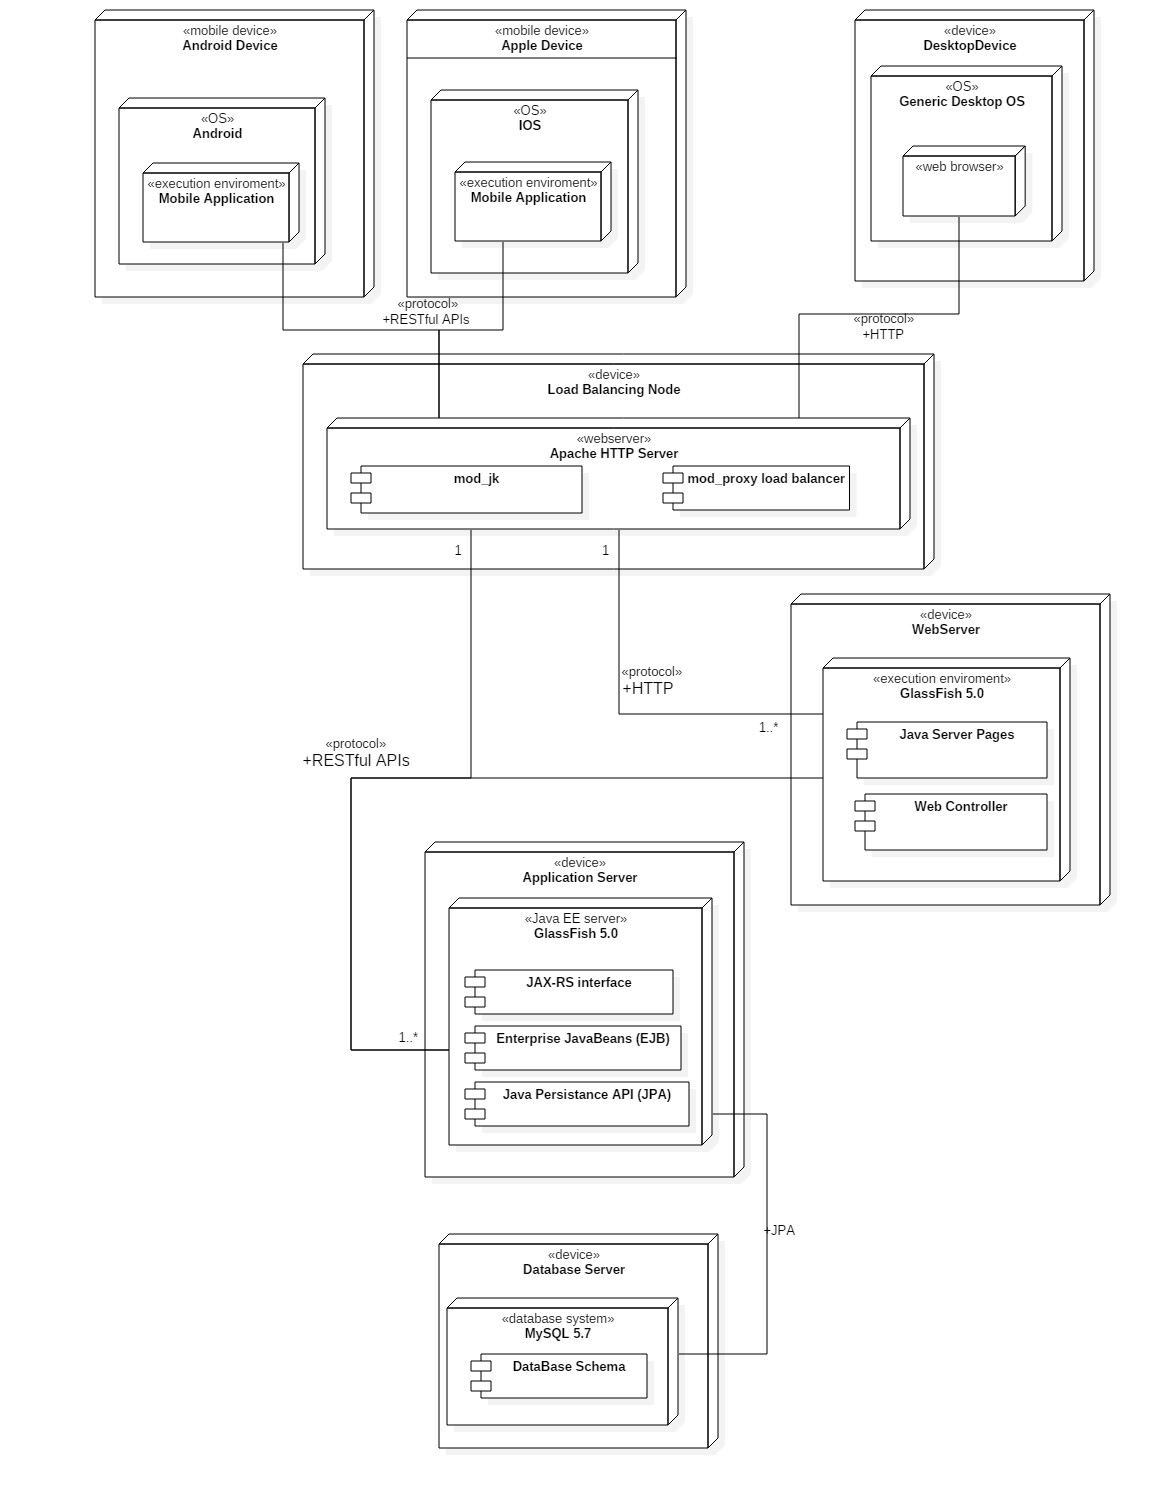
\includegraphics[scale=0.35]{DeploymentDiagram.png}
\end{center}
\caption{Deployment diagram}
\end{figure}

\subsection{Recommended Implementation Choices}
\label{subsect:Recommended Implementation Choices}
Here we provide a set of recommended implementation choices in order to actually develop the Travlendar+ system.
\begin{itemize}
	\item The \textbf{Database Server} may be implemented with MySQL 5.7 as Relational DBMS;
	
	\item The \textbf{Application Server} may be implemented using Java Enterprise Edition (JEE) 8; this choice could allow the developers to focus on the logic to be provided while being supported by reliable APIs and tools, in order to reduce the complexity of the development phase. Using JEE 8 the developers could also guarantee the main non-functional requirements, which are stated in RASD document. The specific JEE 8 choices can be:
	\begin{enumerate}[a)]
		\item GlassFish 5.0 as Application Server implementation;
		\item JPA (Java Persistence API) in order to interact with the database Database Server, in particular Entity Beans can be used to map the data;
		\item EJB (Enterprise Java Beans) in order to implement the business logic, in fact the components described in section \ref{subsect:Application Server} can be implemented as multiple Stateless Session Beans;
		\item JAX-RS in order to implement the interface used through the web with both mobile apps and the web server.
	\end{enumerate}
	
	\item The \textbf{WebServer} may be implemented using Tomcat 8 as HTTP web server implementation and JSP (JavaServer Pages) may be used to provide dynamically generated web pages;
	
	\item The \textbf{Load Balancing Node} may be implemented using an Apache HTTP Server;
	
	\item The \textbf{Android App} may be implemented using Java and XML programming languages;
	
	\item The \textbf{IOS App} may be implemented using Swift programming language.
\end{itemize}
\newpage